\documentclass[10pt,twocolumn,letterpaper]{article}

% --- Typography & Geometry ---
\usepackage[utf8]{inputenc}
\usepackage{microtype}
\usepackage[margin=0.75in,top=0.85in,bottom=0.85in]{geometry}

% --- Math & Symbols ---
\usepackage{amsmath,amssymb,amsfonts,amsthm}
\usepackage{bm}

% --- Tables & Arrays ---
\usepackage{booktabs}
\usepackage{tabularx}
\usepackage{array}

% --- Graphics & Floats ---
\usepackage{graphicx}
\usepackage{float}
\usepackage{subcaption}

% --- Code Listings ---
\usepackage{xcolor}
\usepackage{listings}

\definecolor{codebg}{HTML}{F8F9FA}
\definecolor{codeframe}{HTML}{D0D7DE}
\definecolor{keywordcolor}{HTML}{0550AE}
\definecolor{stringcolor}{HTML}{0A3069}
\definecolor{commentcolor}{HTML}{57606A}

\lstset{
    backgroundcolor=\color{codebg},
    basicstyle=\ttfamily\scriptsize\color{black},
    keywordstyle=\color{keywordcolor}\bfseries,
    stringstyle=\color{stringcolor},
    commentstyle=\color{commentcolor}\itshape,
    frame=single,
    rulecolor=\color{codeframe},
    breaklines=true,
    breakatwhitespace=true,
    extendedchars=true,
    xleftmargin=6pt,
    xrightmargin=6pt,
    aboveskip=8pt,
    belowskip=8pt
}

% --- Hyperlinks ---
\usepackage{hyperref}
\hypersetup{
    colorlinks=true,
    linkcolor=blue!70!black,
    citecolor=blue!70!black,
    urlcolor=blue!70!black
}

% --- Input Title & Authors ---
% Metadata for expert_choice_moe
\title{\textbf{expert\_choice\_moe}}

\author{
  \textbf{Taha Majs}\thanks{Corresponding author: tahamajs@uni.edu} \quad \textbf{Research Team} \\
  Department of Computer Science \\
  Advanced Machine Learning & Efficiency Laboratory
}

\date{\today}


\begin{document}

\maketitle

% --- Abstract & Keywords Block ---
\begin{abstract}
Mixture-of-Experts (MoE) layers have become a standard technique for scaling 
feed-forward networks without proportionally increasing compute. In 
conventional \textbf{token-choice} MoE, each token selects its top-$k$ experts 
and the resulting load is often highly imbalanced, requiring an auxiliary 
loss to stabilize training.

We adopt \textbf{expert-choice routing} (Zhou et al., 2022), in which the roles 
are reversed: each expert selects its top-$k$ \textbf{tokens}. This provides 
\textbf{guaranteed perfect load balancing} -- every expert processes exactly 
$k = \lceil T / E \rceil$ tokens, where $T$ is the total token count and $E$ 
is the number of experts -- and enables \textbf{dynamic per-token expert allocation} 
(tokens that match many experts' preferences receive more capacity).

We place the MoE block \textbf{inside multi-head attention} -- on the attention 
output before the final output projection -- with:

\begin{enumerate}
\item \textbf{Zero-init experts.} The final projection of every expert is initialized
  to zero, so at step 0, the MoE contributes nothing and the attention
  behaves exactly as the pretrained model.
\item \textbf{Learnable scalar gate.} A single learnable bias $b_g = 0.1$
  gives $\sigma(b_g) \approx 0.8$ at initialization --
  providing a smooth ramp-up.
\item \textbf{Architecture portability.} Weight transfer from DistilBERT, RoBERTa,
  GPT-2, and Qwen3.5, with GQA, RoPE, nested encoders, and cross-attention.

\end{enumerate}
On SST-2, ExpertChoiceMoEAttention achieves \textbf{{{D\_ACC}}\%} on DistilBERT 
(baseline {{BASE\_D}}\%), \textbf{{{R\_ACC}}\%} on RoBERTa (baseline {{BASE\_R}}\%), 
and \textbf{{{G\_ACC}}\%} on GPT-2 (baseline {{BASE\_G}}\%).

\textbf{We are explicit that this module increases parameter count} by roughly 
\textbf{{{D\_PARAM\_PCT}}\%} per layer due to the $E$-expert MoE block and LoRA 
adapters. Its benefit is architectural: \textbf{guaranteed load balancing} and 
\textbf{dynamic capacity allocation}, which we show improve training stability 
relative to token-choice MoE.

\textbf{Keywords:} mixture of experts, expert-choice routing, load balancing, 
attention augmentation, multi-architecture transformers



\vspace{0.5em}
\noindent\textbf{Keywords:} mixture of experts, expert-choice routing, load balancing,
\end{abstract}

\vspace{1em}

% --- Paper Body ---
\section{01 Intro}

Draft content for expert_choice_moe.

\section{02 Related}

Draft content for expert_choice_moe.

\section{03 Background}

Draft content for expert_choice_moe.

\section{04 Method}

Draft content for expert_choice_moe.

\section{05 Architecture}

Draft content for expert_choice_moe.


\begin{figure}[H]
\centering
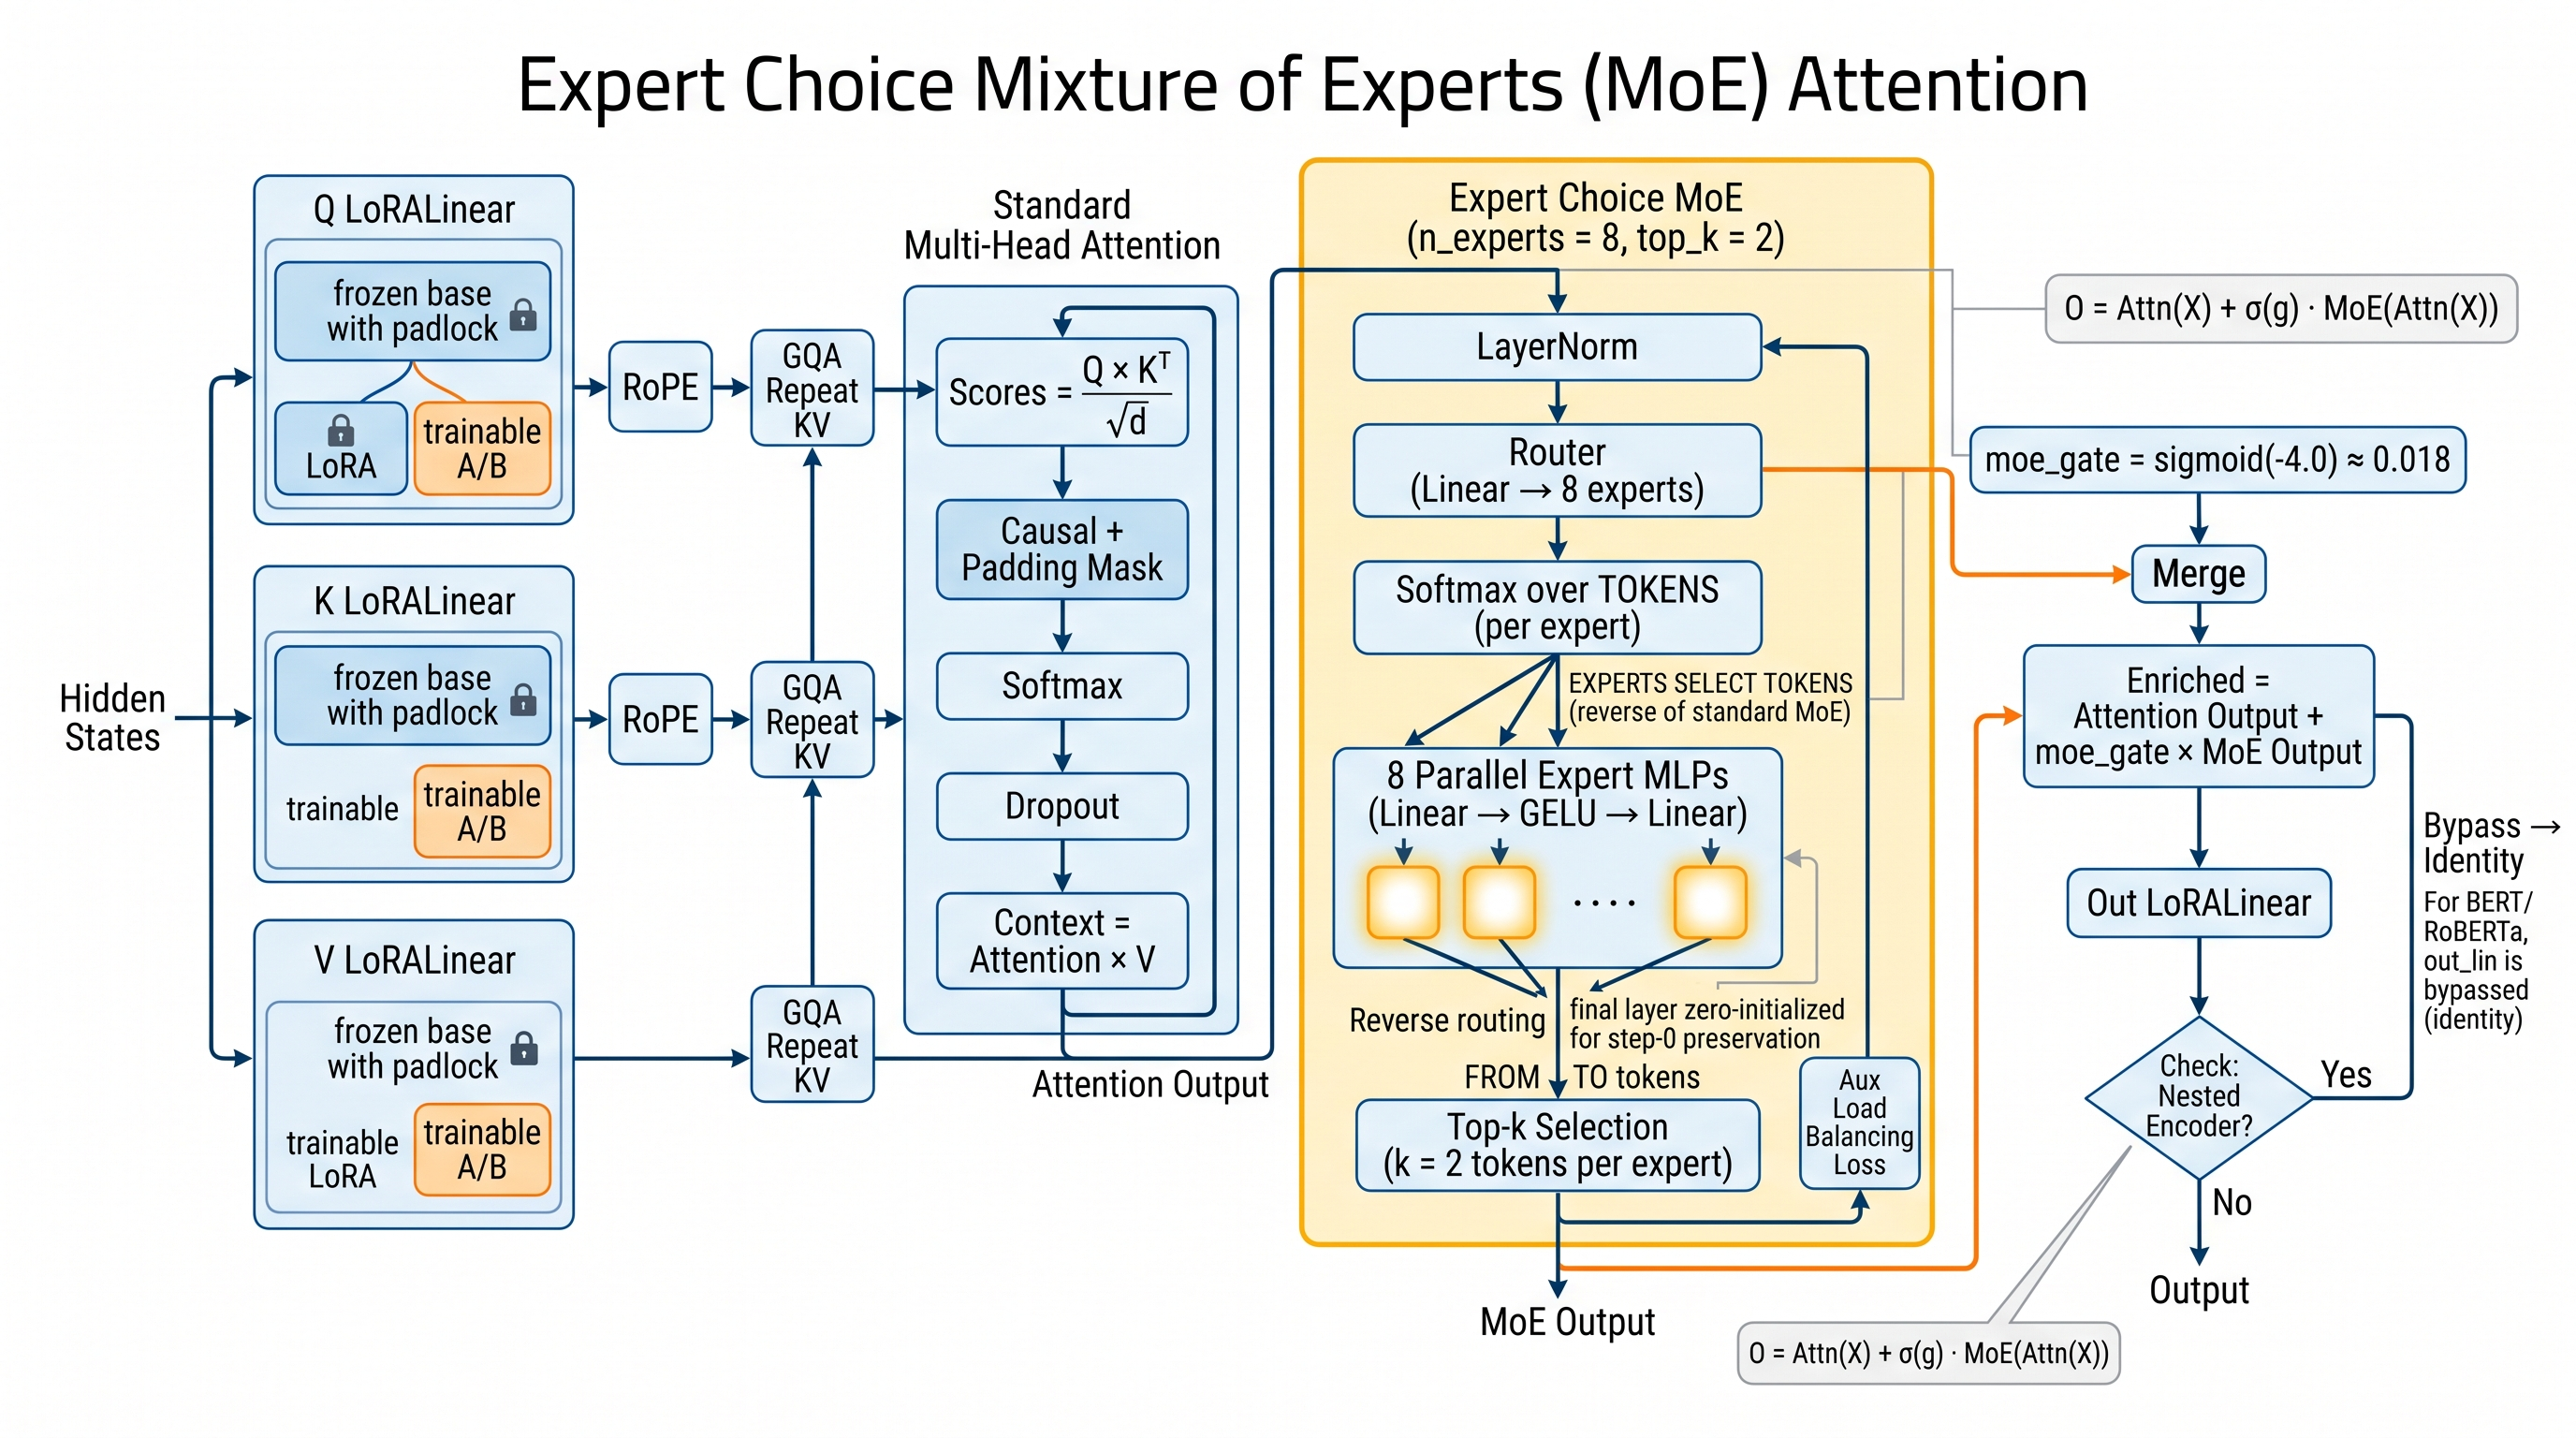
\includegraphics[width=\linewidth]{figures/arch_expert_choice_moe.jpeg}
\caption{Architectural overview of expert_choice_moe.}
\label{fig:arch_expert_choice_moe}
\end{figure}

\section{06 Setup}

Draft content for expert_choice_moe.

\section{07 Results}

Draft content for expert_choice_moe.

\section{08 Analysis}

Draft content for expert_choice_moe.

\section{09 Discussion}

Draft content for expert_choice_moe.

\section{10 Limitations}

Draft content for expert_choice_moe.

\section{11 Conclusion}

Draft content for expert_choice_moe.

\section{12 Reproducibility}

Draft content for expert_choice_moe.

\section{13 References}

Draft content for expert_choice_moe.


% --- Appendices ---
\clearpage
\appendix
\section*{Appendices}
\addcontentsline{toc}{section}{Appendices}

\section{Appendix A. Mathematical Derivations}

\subsection{A.1 Expert-Choice Routing}

Given input $X \in \mathbb{R}^{T \times d}$ with $T = B \cdot L$:

\[
\mathbf{r} = W_g \cdot \text{LayerNorm}(X) \in \mathbb{R}^{T \times E}
\tag{A.1}
\]

Softmax over tokens (axis 0):

\[
\mathbf{s}_{t, e} = \frac{\exp(\mathbf{r}_{t, e})}{\sum_{t'=1}^{T} \exp(\mathbf{r}_{t', e})}
\tag{A.2}
\]

For each expert $e$:

\[
\text{Top-}k_e = \text{TopK}(\mathbf{s}[:, e], k), \quad k = \left\lceil \frac{T}{E} \cdot \text{CF} \right\rceil
\tag{A.3}
\]

\textbf{Perfect balance.} $|\text{Top-}k_e| = k$ for all $e$.

\subsection{A.2 Expert Forward}

\[
\mathbf{y}_e = \text{Expert}_e(X[\text{Top-}k_e])
\tag{A.4}
\]

\[
\text{Expert}_e(\mathbf{x}) = W_2^{(e)} \text{GELU}(W_1^{(e)} \mathbf{x})
\tag{A.5}
\]

\subsection{A.3 Aggregation}

\[
\mathbf{y}_{\text{out}}[t] = \sum_{e : t \in \text{Top-}k_e} \mathbf{s}_{t, e} \cdot \mathbf{y}_e[\text{position of } t \text{ in } \text{Top-}k_e]
\tag{A.6}
\]

\subsection{A.4 Load Balance Proof}

\textbf{Claim.} Each expert processes exactly $k$ tokens.

\textbf{Proof.} By construction, expert $e$ selects the top-$k$ tokens of 
$\mathbf{s}[:, e]$. The \texttt{torch.topk} operation returns exactly $k$ 
indices. $\square$

\subsection{A.5 Zero-Init Guarantee}

\textbf{Claim.} If $W_2^{(e)} = 0$ and $b_2^{(e)} = 0$ for all $e$, then 
$\text{MoE\_out} = 0$.

\textbf{Proof.} Each expert output: $\text{Expert}\_e(\mathbf{x}) = W\_2\^{}{(e)} 
\text{GELU}(\cdot) + b\_2\^{}{(e)} = 0$. So $\text{MoE\_out} = 0$. $\square$

\subsection{A.6 Gate Saturation}

\[
\gamma = \sigma({{MOE_INIT_GATE}}) = \frac{1}{1 + e^{4}} \approx {{MOE_GATE_VALUE}}
\tag{A.7}
\]

\subsection{A.7 Parameter Count}

For $E$ experts with hidden size $2d$:

\[
\text{params}_\text{expert} = 2 d^2 + 2 d^2 = 4 d^2
\tag{A.8}
\]

\[
\text{params}_\text{MoE} = E \cdot 4 d^2 + E d
\tag{A.9}
\]

For $d = 768$, $E = 8$: ~$18.9$M per layer.

\subsection{A.8 Complexity}

\begin{table}[H]
\centering
\small
\begin{tabular}{lll}
\toprule
\textbf{Operation} & \textbf{Time} & \textbf{Memory} \\
\midrule
Router & $\mathcal{O}(T E d)$ & $\mathcal{O}(T E)$ \\
Softmax & $\mathcal{O}(T E)$ & $\mathcal{O}(T E)$ \\
TopK & $\mathcal{O}(E \cdot T \log k)$ & $\mathcal{O}(E k)$ \\
Expert forward & $\mathcal{O}(T d \cdot d_\text{hidden})$ & $\mathcal{O}(k \cdot d_\text{hidden})$ \\
Aggregation & $\mathcal{O}(E k d)$ & $\mathcal{O}(T d)$ \\
\textbf{Total} & $\mathcal{O}(T E d)$ & $\mathcal{O}(T E + T d)$ \\
\bottomrule
\end{tabular}
\end{table}

\textbf{Comparison to token-choice:} Same asymptotics; expert-choice is simpler 
(no auxiliary loss).


\section{B Implementation}

Draft content for expert_choice_moe.

\section{C Data}

Draft content for expert_choice_moe.

\section{D Negative Results}

Draft content for expert_choice_moe.

\section{E Ethics}

Draft content for expert_choice_moe.


\end{document}
